%!TEX program = xelatex

% \documentclass[notes]{beamer}
% \documentclass[notes=only]{beamer}
\documentclass{beamer}

% Good bibliography
\RequirePackage[backend=biber]{biblatex}
\addbibresource[datatype=bibtex]{biblio.bib}

% Icon Fonts
\RequirePackage{academicons}
\RequirePackage{fontawesome5}

% Correct the path when including svg pictures
\RequirePackage{import}

% For nice verbatim
\RequirePackage{minted}

% To resize graphic and table
\RequirePackage{graphics}

% For captions
\RequirePackage{caption}

% Arrange theme
\usetheme[
	progressbar=frametitle,
	sectionpage=none,
	numbering=fraction
]{metropolis}

% Color the progress:
% - green for SciLifeLab
% - violet for KI
\setbeamercolor{progress bar}{fg=green,bg=white}

\author{Maxime Garcia\\ \faTwitter\ @gau\\ \faGithub\ @MaxUlysse\\ \faGlobe\ https://maxulysse.github.io/}
\date{2018-01-31}
\title{Running CAW with AWS Batch}
\titlegraphic{\hfill
\includegraphics[height=1cm]{pictures/CAW}}
\subtitle{Hopefully my last talk about CAW ever...}
\institute{SciLifeLab NGI / BarnTumörBanken\\ % Don't forget logos
	\vfill
	
\includegraphics[height=.7cm]{pictures/SciLifeLab}
	\hfill
	
\includegraphics[height=.7cm]{pictures/NGI}
	\hfill
	
\includegraphics[height=.7cm]{pictures/NBIS}
	\hfill
	
\includegraphics[height=.7cm]{pictures/KI}
	\hfill
	
\includegraphics[height=.7cm]{pictures/KTH}
	\hfill
	
\includegraphics[height=.7cm]{pictures/SU}
	\hfill
	
\includegraphics[height=.7cm]{pictures/UU}
	\hfill
	\includegraphics[height=.7cm]{pictures/Barntumörbanken-logo}
}

\begin{document}

\maketitle

\section{CAW}

\begin{frame}{Definition}
	\begin{center}
		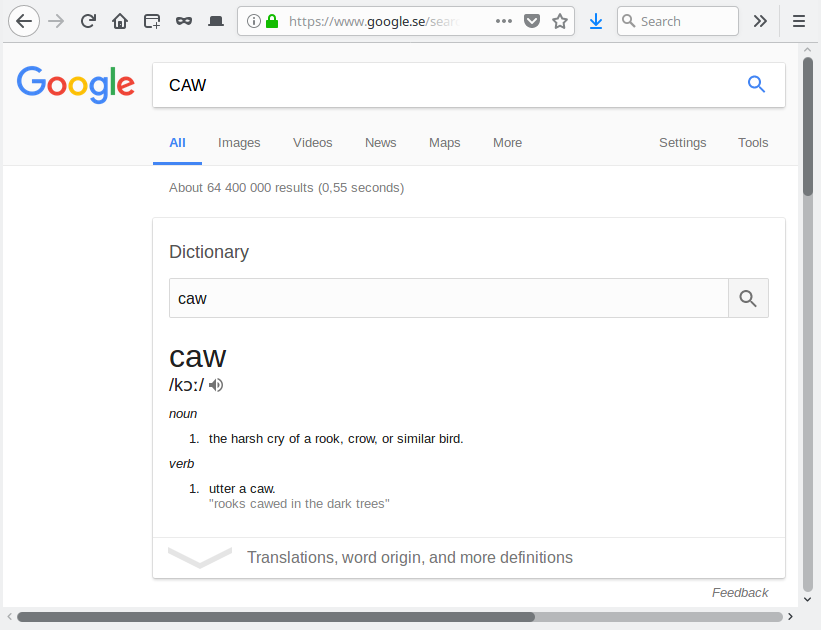
\includegraphics[height=7cm]{pictures/Definition.png}
	\end{center}
\end{frame}

\begin{frame}{What is CAW?}
	\vfill
	\begin{center}
		
\includegraphics[height=1cm]{pictures/CAW}
		\captionof*{figure}{\faGlobe\ http://opensource.scilifelab.se/projects/caw/}
	\end{center}
	\begin{itemize}
		\item Nextflow pipeline
		\item<2-> Developed at NGI
		\item<3-> In collaboration with NBIS
		\item<4-> Support of The Swedish Pediatric Tumor Biobank
	\end{itemize}
	\begin{center}
		
\includegraphics[height=1cm]{pictures/NGI}<2->
		\only<2->{\hfill}
		\includegraphics[height=1cm]{pictures/Barntumörbanken-logo}<4->
		\only<3->{\hfill}
		
\includegraphics[height=1cm]{pictures/NBIS}<3->
	\end{center}
	\vfill
\end{frame}

\begin{frame}{What does CAW do?}
	\begin{center}
		
\includegraphics[height=1cm]{pictures/CAW}
	\end{center}
	\pause
	\begin{itemize}
		\item WGS analysis (Tumor/Normal pair or Germline)
		\pause
		\item Handles both GRCh37 and GRCh38
		\pause
		\item Based on GATK best practices for processing FASTQ files
		\pause
		\item<5-> SNPs, SNVs and indels
		\begin{itemize}
			\item<6-> MuTect1, MuTect2, Strelka, and GATK HaplotyeCaller
		\end{itemize}
		\pause
		\item<7-> Structural variants
		\begin{itemize}
			\item<8-> Manta
		\end{itemize}
		\pause
		\item<9-> Heterogeneity, ploidy and CNVs
		\begin{itemize}
			\item<10-> ASCAT
		\end{itemize}
		\pause
		\item<11-> Containers (portable, reproducible)
		\begin{itemize}
			\item<12-> Docker or Singularity
		\end{itemize}
	\end{itemize}
\end{frame}

\section{Is there more?}

\begin{frame}{Where to use CAW?}
	\begin{center}
		\only<2-5>{
\includegraphics[height=2cm]{pictures/uppmax.png}}
		\only<6>{
\includegraphics[height=3cm]{pictures/AWS}}
		\only<7>{
\includegraphics[height=8cm]{pictures/Wonka-meme.png}}
	\end{center}
	\begin{itemize}
		\item<1> Any POSIX compatible system
		\pause
		\item<-5> Rackham
		\pause
		\item<-5> Bianca
		\pause
		\item<-5> Irma
		\pause
		\item<6> AWS Batch
	\end{itemize}
\end{frame}

\begin{frame}[fragile]{CAW with AWS Batch}
	\begin{center}
		
\includegraphics[height=2cm]{pictures/Batch.png}
	\end{center}
	\pause
	\begin{itemize}
		\item A single command line
	\end{itemize}
	\begin{minted}[fontsize=\scriptsize]{bash}
nextflow run main.nf -profile awsbatch -w s3://caw-test-results/work \
--genome smallGRCh37 --sample s3://caw-test-data/tsv/tiny-s3.tsv \
--outDir s3://caw-test-results/Results
	\end{minted}
	\pause
	\footnotesize
	\faGlobe\ https://maxulysse.github.io/2017/11/16/Running-CAW-with-AWS-Batch/
\end{frame}

\begin{frame}{Going further}
	\begin{center}
		
\includegraphics[height=2cm]{pictures/Batch.png}
	\end{center}
	\begin{itemize}
		\item Run a full size test sample
		\pause
		\item Gather reports
		\pause
		\item Get a pricing
		\pause
		\item Wait for Amazon to finally come to Stockholm
	\end{itemize}
\end{frame}

\section{Acknowledgments}

\begin{frame}{The List of People Involved}
	\begin{table}
		\resizebox{.8\textwidth}{!}{%
		\begin{tabular}{ll}
			Sebastian DiLorenzo &	Markus Mayrhofer \\
			Jesper Eisfeldt 		&	Monica Nistèr \\
			Phil Ewels					& Björn Nystedt \\
			Maxime Garcia 			&	Pall Olason \\
			Szilveszter Juhos 	&	Markus Ringnér \\
			Max Käller 					&	Pelin Sahlén \\
			Malin Larsson 			&	Johanna Sandgren \\
			Marcel Martin 			&	Teresita Díaz De Ståhl \\
		\end{tabular}}
	\end{table}
\end{frame}

\begin{frame}[fragile]{Where to find us?}
	\begin{itemize}
		\item We are on the SciLifeLab Slack
		\faSlack \mint[fontsize=\small]{html}|#cancer-pipeline|
		\pause
		\item We have a gitter channel
		\faGitter \mint[fontsize=\small]{html}|https://gitter.im/SciLifeLab/CAW|
		\pause
		\item Our code is hosted on Github
		\faGithub \mint[fontsize=\small]{html}|https://github.com/SciLifeLab/CAW|
	\end{itemize}
\end{frame}

\usebackgroundtemplate{
	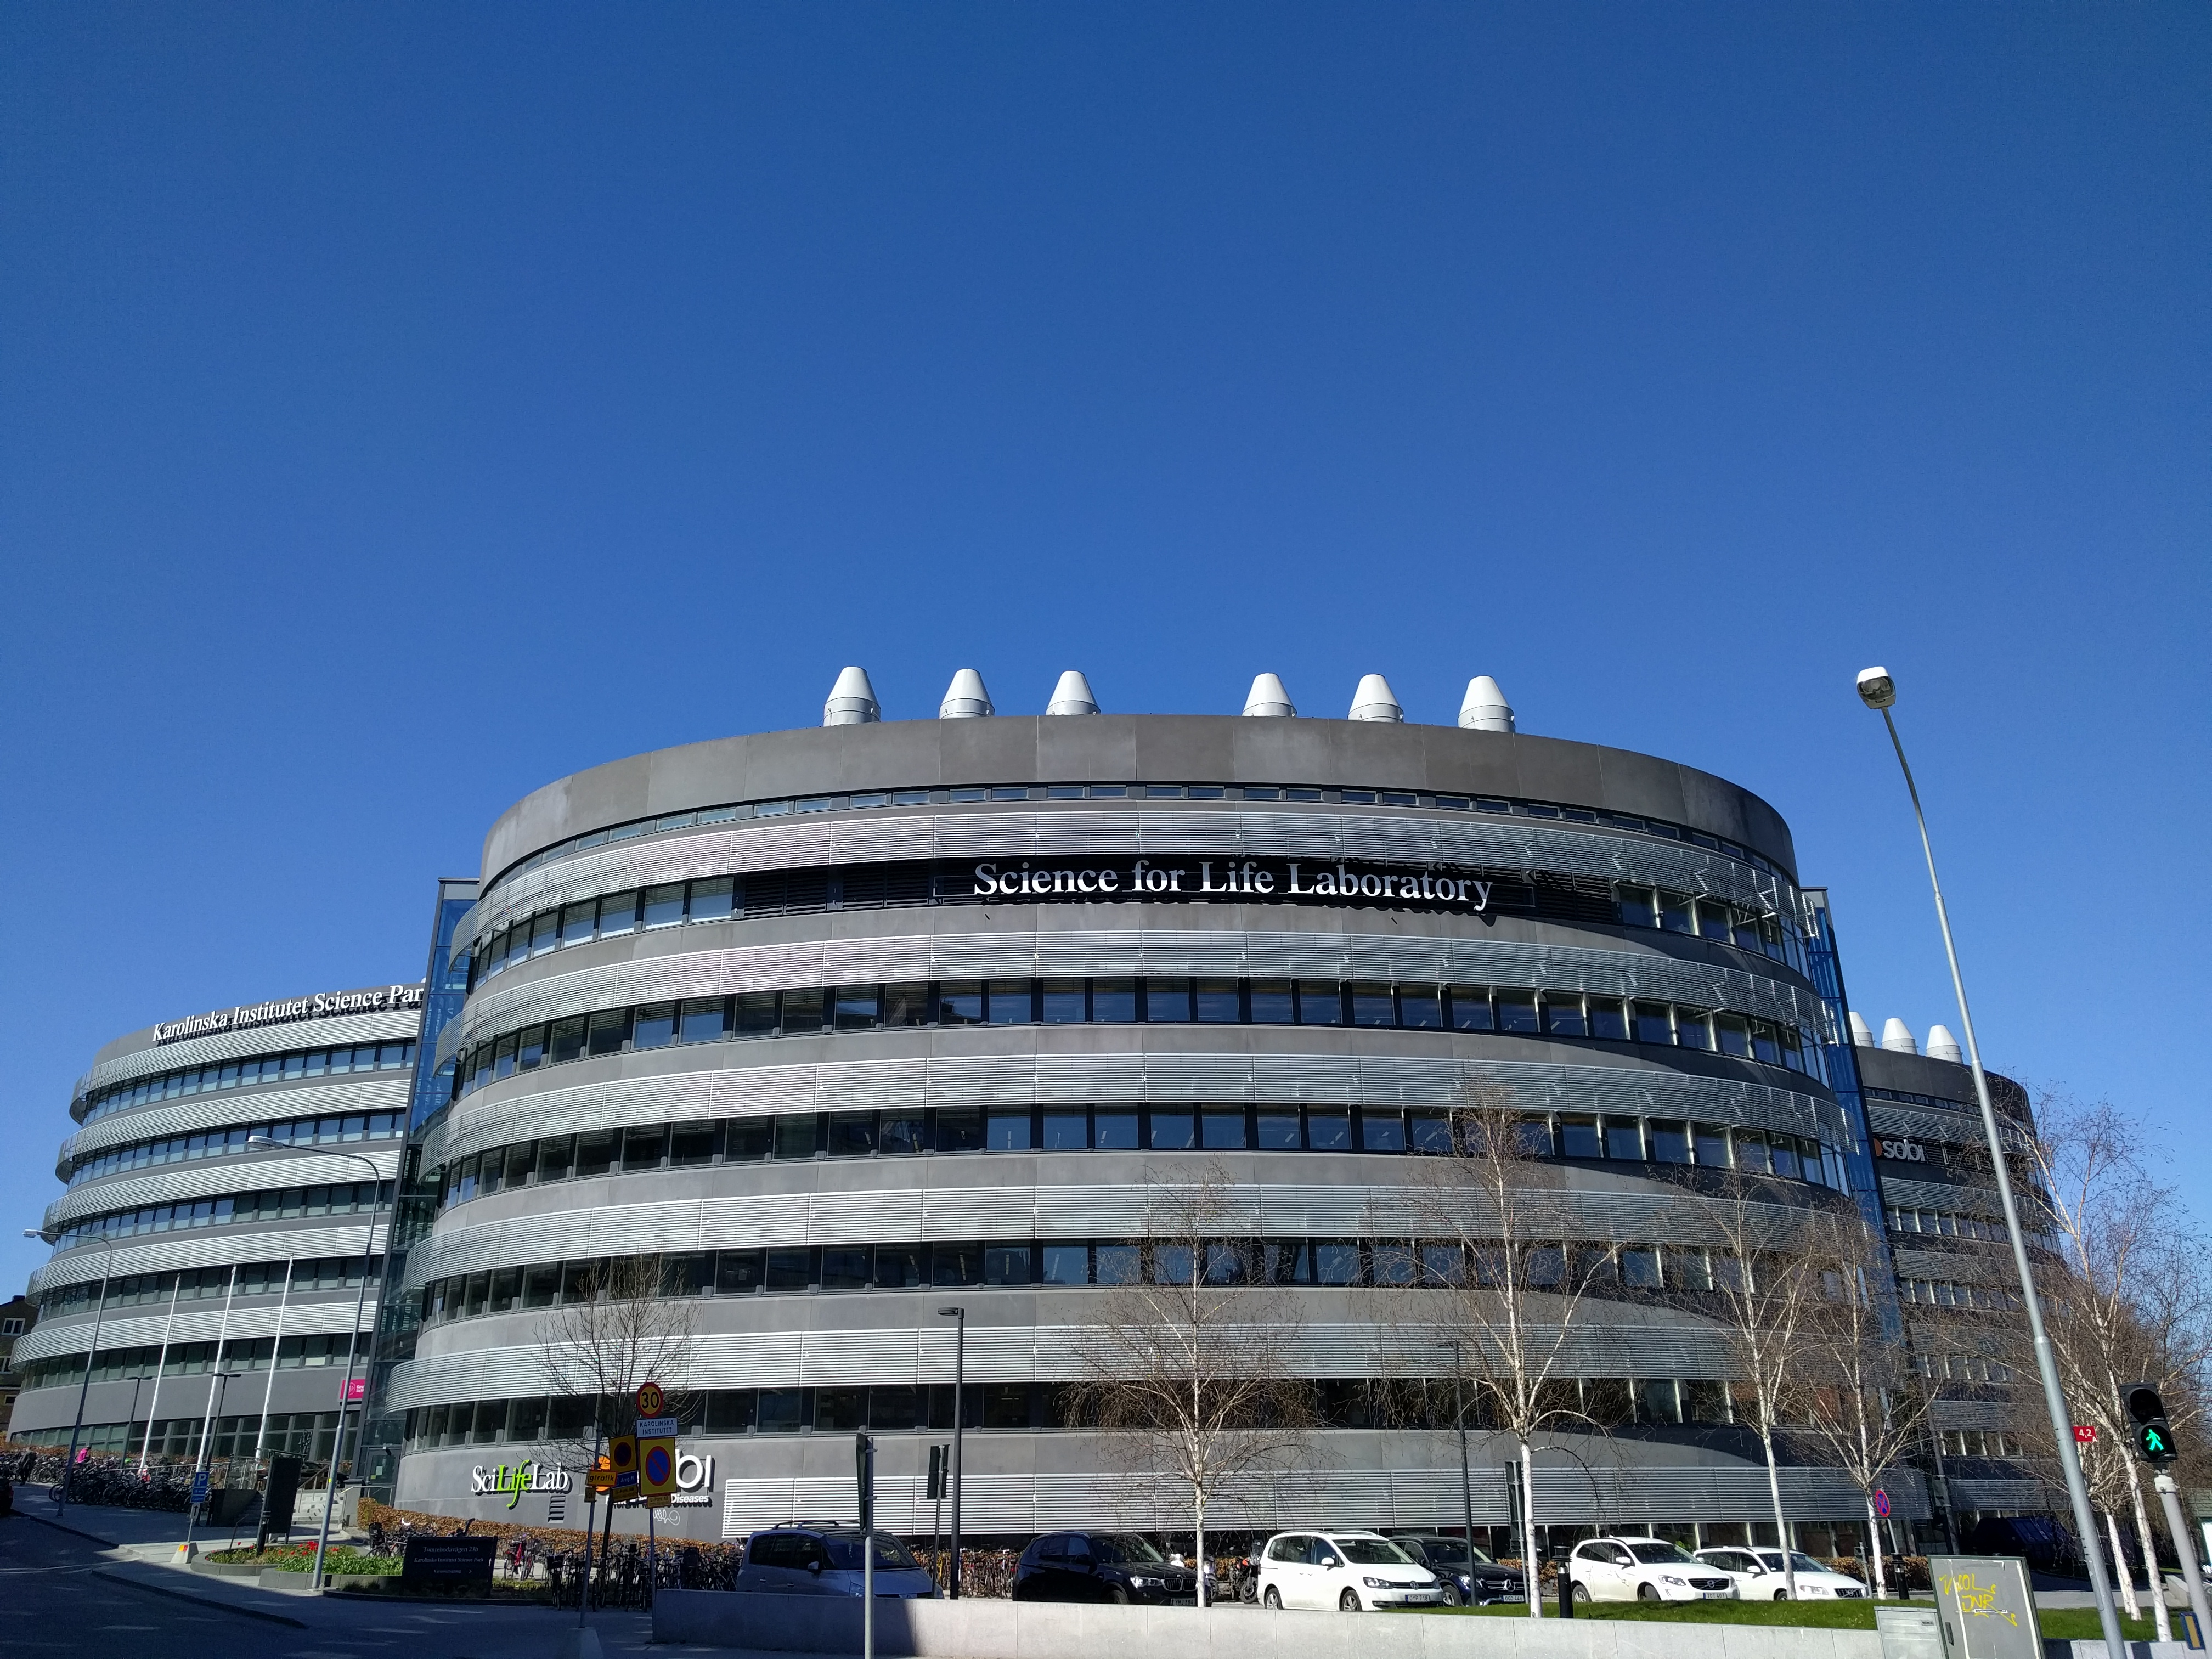
\includegraphics[width=\paperwidth]{pictures/SciLifelab-BlueSky.jpg}
}

\begin{frame}[plain,noframenumbering]{Any questions?}
\end{frame}

\end{document}
